\subsubsection{Acopladores ópticos}

% SLIDE DE ACOPLADORES ÓPTICOS
\begin{frame}
\frametitle{Acopladores ópticos}

A aplicação dentro do projeto é o isolamento elétrico que pode ser estabelecido entre os circuitos de controle de potência, protegendo os circuitos sensíveis a uma alta tensão como a placa controladora Arduino.

\begin{figure}
\centering
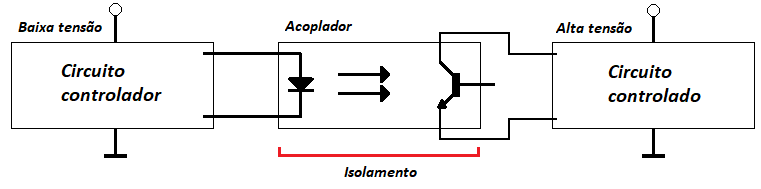
\includegraphics[scale = 0.5]{figs/acoplador}
\end{figure}

\begin{figure}
\centering
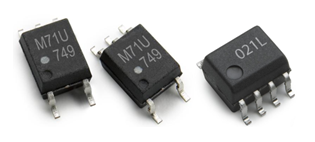
\includegraphics[scale = 0.7]{figs/fotoacoplador}
\end{figure}

\end{frame}
